\documentclass{beamer}

\usepackage{color,fancyvrb}

\usetheme{Pittsburgh}

\title{Improving marginpars and floats}
\author{Stephen Hicks}
\date{29 June 2010}

\DefineShortVerb{\|}

%% \def\sidebyside#1{{%
%%   \catcode`\$0\catcode`\^1\catcode`\&2%
%%   $catcode`$\12$catcode`${12$catcode`$}12%
%%   $obeylines$obeyspaces$ttfamily
%%   $input #1
%% &}

\begingroup\obeylines\gdef\col
#1\uncol
{{\color{red}#1}}\endgroup

\def\gobble#1{}
\def\cs#1{\texttt{\expandafter\string\csname#1\endcsname}}
\def\lit#1{\expandafter\gobble\string#1}

\def\inputsrc#1{{%
  \catcode`\\12\catcode`\{12\catcode`\}12\catcode`\%0%
  \obeylines\obeyspaces\ttfamily
  \input #1
}}

\def\sidebyside#1{%
  \hbox to \textwidth{
    \setbox0\vbox to 10pc{%
      \hskip-.05\textwidth
      \vbox to 10pc{%
        \hsize=0.55\textwidth
        \small\inputsrc{#1}%
        \vfill
      }
    }%
    \wd0=0.5\textwidth\box0%
    \fbox{\includegraphics[height=15pc,clip]{#1}}%
  }%
}

\begin{document}

\errorcontextlines=12

\begin{frame}
  \titlepage
\end{frame}

\section*{Outline}
\begin{frame}
  \tableofcontents
\end{frame}

\section{Margins}
\subsection{Introduction}
\begin{frame}[fragile]
  \frametitle{\LaTeX{} deals poorly with long margin notes}
  \sidebyside{margins-bad} % prints source next to product...
  %\inputsrc{margins-bad}
  \vskip-1pc Why shouldn't this ``just work''?
\end{frame}

\begin{frame}
  \frametitle{What we expected\ldots}
  \sidebyside{margins-bad-expected}
\end{frame}

\begin{frame}[fragile]
  \frametitle{Common workaround}
  \begin{block}{Last-minute \cs{vskip} tweaks}
    \begin{itemize}
    \item |\marginpar{|{\color{red}|\vskip-30pc|}\ldots|}|
    \item {\color{red}|\mparshift30pc|}|\marginpar{|\ldots|}|
      \begin{itemize}
      \item (custom macro to insert the |\vskip|)
      \end{itemize}
    \item time-consuming to determine correct skips
    \item broken whenever page breaks change
    \item motivation: Ruina/Pratap dynamics text
    \end{itemize}
  \end{block}
\end{frame}

\begin{frame}
  \frametitle{\LaTeX's \cs{marginpar} macro\\\normalsize
  (\texttt{ltfloat.dtx} and \texttt{ltoutpout.dtx})}
  \begin{block}{\cs{marginpar} (in outer horizontal mode)}
    \begin{itemize}
    \item store the note in a float box (actually, two)
    \item insert two large negative penalties to invoke output routine
    \end{itemize}
  \end{block}
  \begin{block}{\cs{output} routine}
    \begin{itemize}
    \item keeps track of bottom of previous margin note
    \item looks at \cs{@pageht} to determine current vertical position
    \item immediately places the margin box at the lower of the two
    \end{itemize}
  \end{block}
  \structure{%
    (Usually) prevents intersection, but allows falling through bottom}
\end{frame}
 
\begin{frame}
  \frametitle{A different approach\\\normalsize(devised by Andy Ruina)}
  \begin{block}{Goals: margin notes should\ldots}
    \begin{itemize}
    \item fit on the page without intersecting
    \item be as close as possible to callout locations
    \item float to subsequent pages if necessary
    \end{itemize}
  \end{block}
  \begin{block}{Strategy}
    \begin{enumerate}
      \addtocounter{enumi}{-1}
    \item save all margin notes in float boxes until whole page builds
    \item try to put each box at the proper location
      \begin{itemize}
      \item keep track of total box height so we know when we're full
      \end{itemize}
    \item push boxes down so they don't intersect
    \item push boxes up so they don't fall off bottom
    \end{enumerate}
  \end{block}
\end{frame}

\begin{frame}[fragile]
  \frametitle{Implementation}
  \begin{itemize}
  \item |\newtoks\marginlist|
    \vskip0.5pc
  \item In |\output| routine after a |\marginpar|{\small (via |\@addmarginpar|)},
    \begin{itemize}
    \item Append |\note{text}{\@pageht}| to |\marginlist|
    \end{itemize}
    \vskip0.5pc
  \item In page-building |\output| routine{\small (via |\@combinefloats|)},
    \begin{itemize}
    \item Run |\marginlist| with |\note=\note@down| keeping track of
      bottom of last note and total vertical space, and adding notes
      and ``glue'' back to |\marginlist| (in reverse) or a deferral
      list if we run out of room
    \item Run |\marginlist| with |\note=\note@up|, removing the glue
      until the bottom of the last note is on the page
    \item Build margin material into box and abut it with main column
    \end{itemize}
  \end{itemize}
\end{frame}

\begin{frame}
  \frametitle{Example\smash{\llap{\lower1.5pc\hbox{\normalsize(step 1)}}}}
  \hbox to 1.1\textwidth{%
    \hskip-.2\textwidth
    \hfill
    \rlap{\vbox{\hsize=0.4\textwidth\begin{itemize}
        \item page of text with 5 marginpars
        \item \LaTeX\ would push 3 and 5 down
        \item 5 would fall off bottom
      \end{itemize}\vskip5pc}}%
    \hphantom{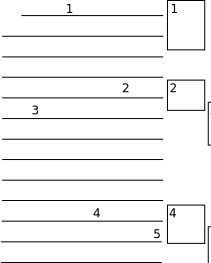
\includegraphics[height=0.6\textheight]{example1}}%
    \hfill
    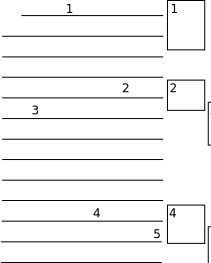
\includegraphics[height=0.6\textheight]{example1}
    \hfill
  }
\end{frame}

\begin{frame}
  \frametitle{Example\smash{\llap{\lower1.5pc\hbox{\normalsize(step 2)}}}}
  \hbox to 1.1\textwidth{%
    \hskip-.2\textwidth
    \hfill
    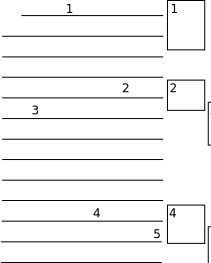
\includegraphics[height=0.6\textheight]{example1}
    \hfill
    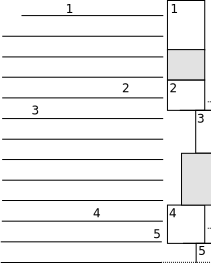
\includegraphics[height=0.6\textheight]{example2}
    \hfill
  }
\end{frame}

\begin{frame}
  \frametitle{Example\smash{\llap{\lower1.5pc\hbox{\normalsize(step 3)}}}}
  \hbox to 1.1\textwidth{%
    \hskip-.2\textwidth
    \hfill
    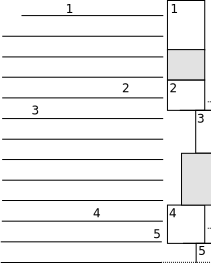
\includegraphics[height=0.6\textheight]{example2}
    \hfill
    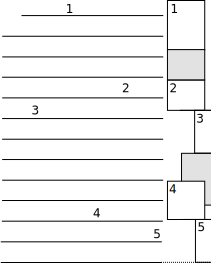
\includegraphics[height=0.6\textheight]{example3}
    \hfill
  }
\end{frame}

\begin{frame}
  \frametitle{Example\smash{\llap{\lower1.5pc\hbox{\normalsize(finished)}}}}
  \hbox to 1.1\textwidth{%
    \hskip-.2\textwidth
    \hfill
    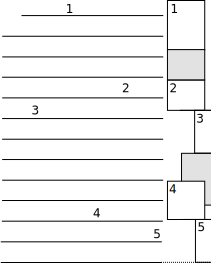
\includegraphics[height=0.6\textheight]{example3}
    \hfill
    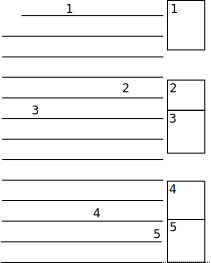
\includegraphics[height=0.6\textheight]{example4}
    \hfill
  }
\end{frame}

\begin{frame}[fragile]
  \frametitle{Beyond the basics}
  \begin{block}{Additional features}
    \begin{itemize}
    \item |\marginparpush| works the same as standard \LaTeX
    \item |\marginskip{|\emph{length}|}| adds an incompressible gap
    \item |\mparshift{|\emph{length}|}| allows adjusting one note's position
    \item |\extendmargin{|\emph{length}|}| makes this page's margin longer
    \item |\clearmargin| stops new material from going into this margin
    \item |\blockmargin|, |\unblockmargin|, |\marginphantom{|\emph{length}|}|
      \vskip-0.3pc
      \begin{itemize}
      \item create gaps in the margin where no material can go
      \item useful for extra-wide figures or equations
      \end{itemize}
    \end{itemize}
  \end{block}
\end{frame}

\begin{frame}
  \frametitle{Floats}
  \begin{block}{While we're at it\ldots}
    \begin{itemize}
    \item margin notes treated internally similar to floats
    \item many people frustrated by unpredictable float behavior
      \begin{itemize}
      \item countless packages (\texttt{placeins}, \texttt{float},
        \texttt{here}, \ldots)
      \item how many know what \texttt{[!]} actually does?
      \end{itemize}
    \item how to deal with figures in the margin?
    \end{itemize}
  \end{block}
\end{frame}

\begin{frame}
  \frametitle{\LaTeX's float routines\\\normalsize(\cs{@addtocurcol})}
  \begin{block}{Reasons floats aren't where they're expected}
    \begin{itemize}
    \item float of the same type already on the deferred list
    \item too many floats or not enough room left on page
    \item not enough text (cf. \cs{textfraction}) but not declared \texttt{[p]}
    \item \texttt{[!]} often doesn't help
    \end{itemize}
  \end{block}
  \vskip 2pc
  Massive confusion when subsequent floats disappear too!
\end{frame}

\begin{frame}
  \frametitle{A better alternative?\\\normalsize(first attempt)}
  \begin{block}{Well, a \emph{simpler} alternative, anyway}
    \begin{itemize}
    \item often users don't care about strictly ordered floats
      \begin{itemize}
      \item (as long as the numbers come out in the right order)
      \end{itemize}
    \item rather than deferring, option to \emph{disorder}/\emph{renumber}
    \item \texttt{[h]} could try harder, forcing a page break if necessary (?)
    \item \texttt{[p]} should always be assumed
    \end{itemize}
  \end{block}
\end{frame}





\begin{frame}
  \frametitle{Concerns/Caveats}
  \begin{block}{Corner cases}
    \begin{itemize}
    \item \LaTeX\ source littered with corner cases, many of which
      I don't understand and probably missed (e.g. \cs{@kludgeins},
        \cs{@bsphack}, \ldots)
    \item currently the margin and float code all tied together:
      still need to separate
    \end{itemize}
  \end{block}
\end{frame}
\end{document}
